% ==========================================
% SEÇÃO DE ANEXOS A SER INCLUÍDA NO FINAL
% ==========================================

\chapter{Anexos}

\begin{figure}[H]
    \centering
    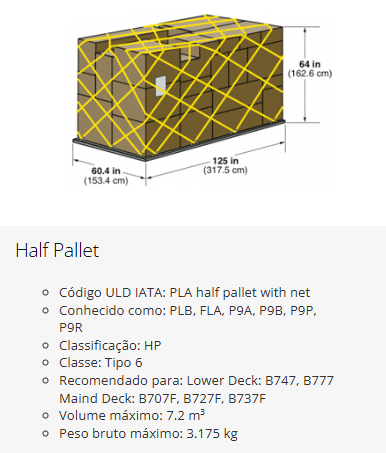
\includegraphics[width=0.5\linewidth]{images/half pallet.png}
    \caption{Palete Padrão\cite{sideral_comex_containers}}
    \label{fig:palete}
\end{figure}

\section{Integrantes do Projeto}

Abaixo segue a lista dos integrantes do projeto e suas respectivas matrículas:

\vspace{0.5cm}

\begin{table}[H]
\centering
\begin{tabular}{ll}
\hline
\textbf{Nome} & \textbf{Matrícula} \\ \hline
Caio Fernandes Rickli Costa & 2020022308 \\
Carolina Chaves Ferrari de Lima & 2021015666 \\
Filipe Gomes Ferreira e Silva & 2022060355 \\
Flaubert Silva Ferreira & -- \\
Gabriel Fernando Duarte Marques & 2022060134 \\
Gabriel Henrique Ferreira Soares & 2019070418 \\
Gabriela Araujo Machado & 2019022367 \\
Luísa Vilela Gonçalves & 2020069380 \\
Pedro Henrique Oliveira Roquette & 2022060410 \\
Pedro Palma Maia Ornelas & 2022095612 \\
Rodrigo Pena Teobaldo & 2022060312 \\
Saulo de Lacerda Pires & 2020022685 \\
Vicente Fernandes de Queiroz Neto & 2022060142 \\
Victor Gomes Teixeira & -- \\
Vitor da Silva Gonçalves & 2022045291 \\
Vitor de Jesus Mendes & 2022421170 \\ \hline
\end{tabular}
\end{table}



\section{Informações adicionais da dinâmica longitudinal}

\subsection{Gráficos CG traseiro}

\begin{figure}[H]
    \centering
    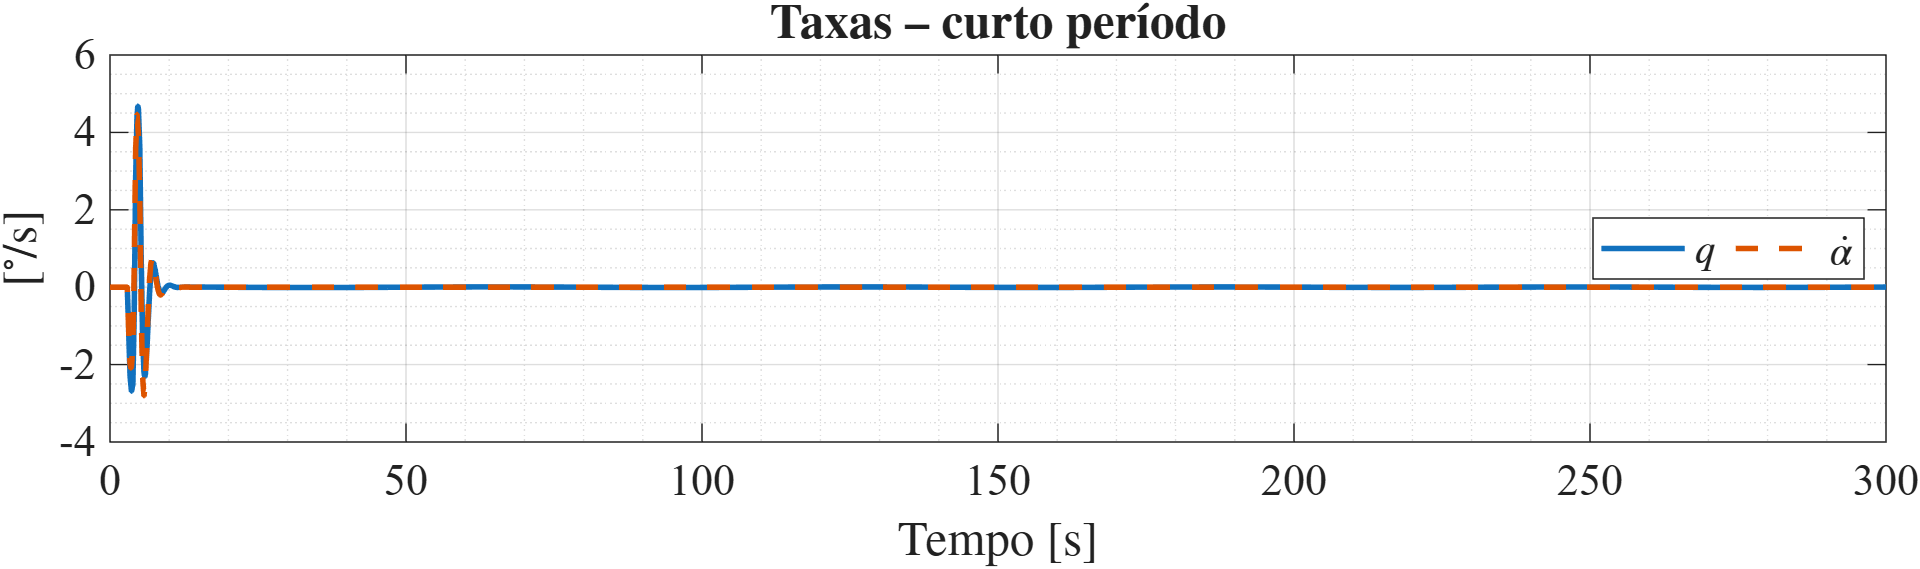
\includegraphics[width=0.9\linewidth]{images/estabilidade/Taxas_CG_traseiro.png}
    \caption{Evolução de q e $\dot{\alpha}$ para CG traseiro}
    \label{fig:placeholder}
\end{figure}

\begin{figure}[H]
    \centering
    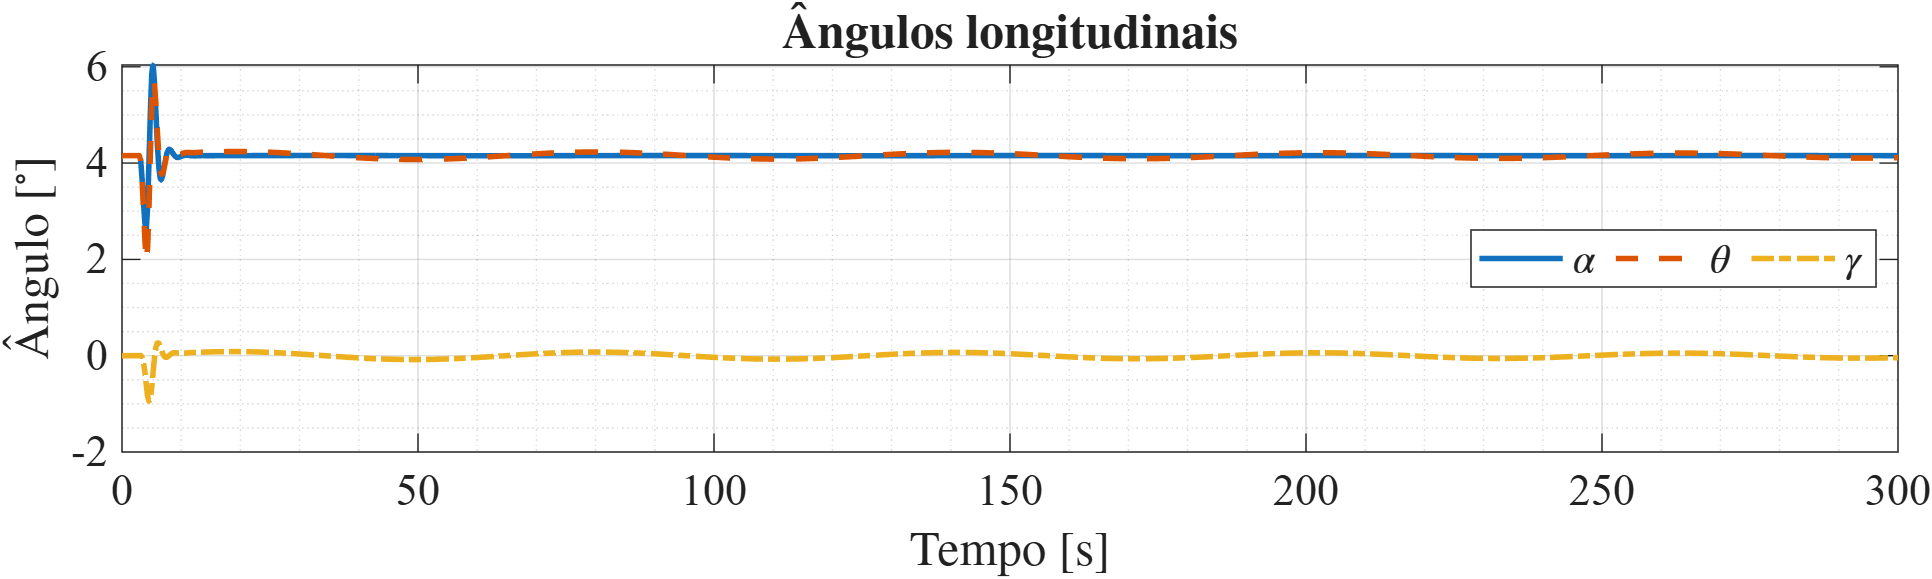
\includegraphics[width=0.9\linewidth]{images/estabilidade/angulos_300s_CG_traseiro.png}
    \caption{Evolução de $\alpha$, $\theta$ e $\gamma$ para CG traseiro}
    \label{fig:placeholder}
\end{figure}

\subsection{Gráficos CG dianteiro}


\begin{figure}[H]
    \centering
    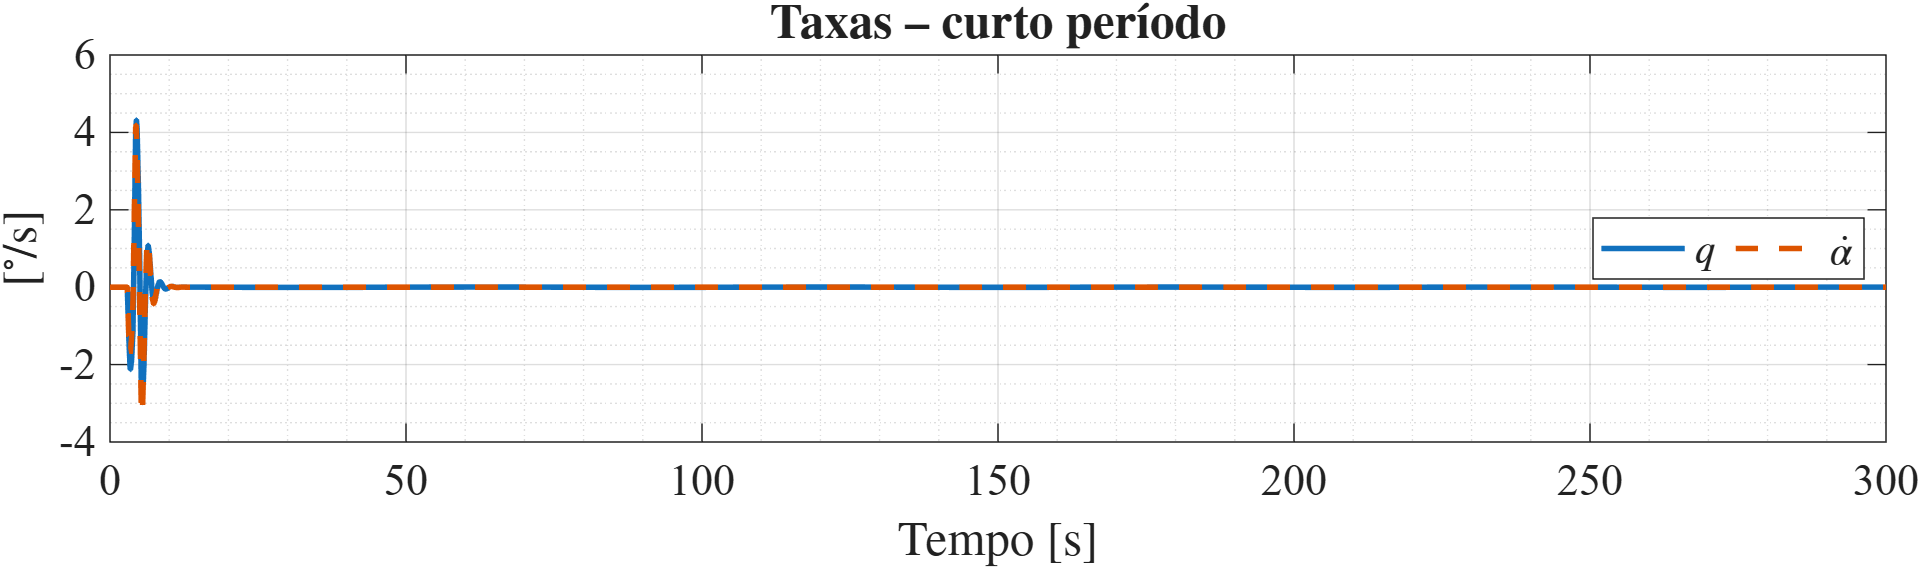
\includegraphics[width=0.9\linewidth]{images/estabilidade/Taxas_CG_dianteiro.png}
    \caption{Evolução de q e $\dot{\alpha}$ para CG dianteiro}
    \label{fig:placeholder}
\end{figure}

\begin{figure}[H]
    \centering
    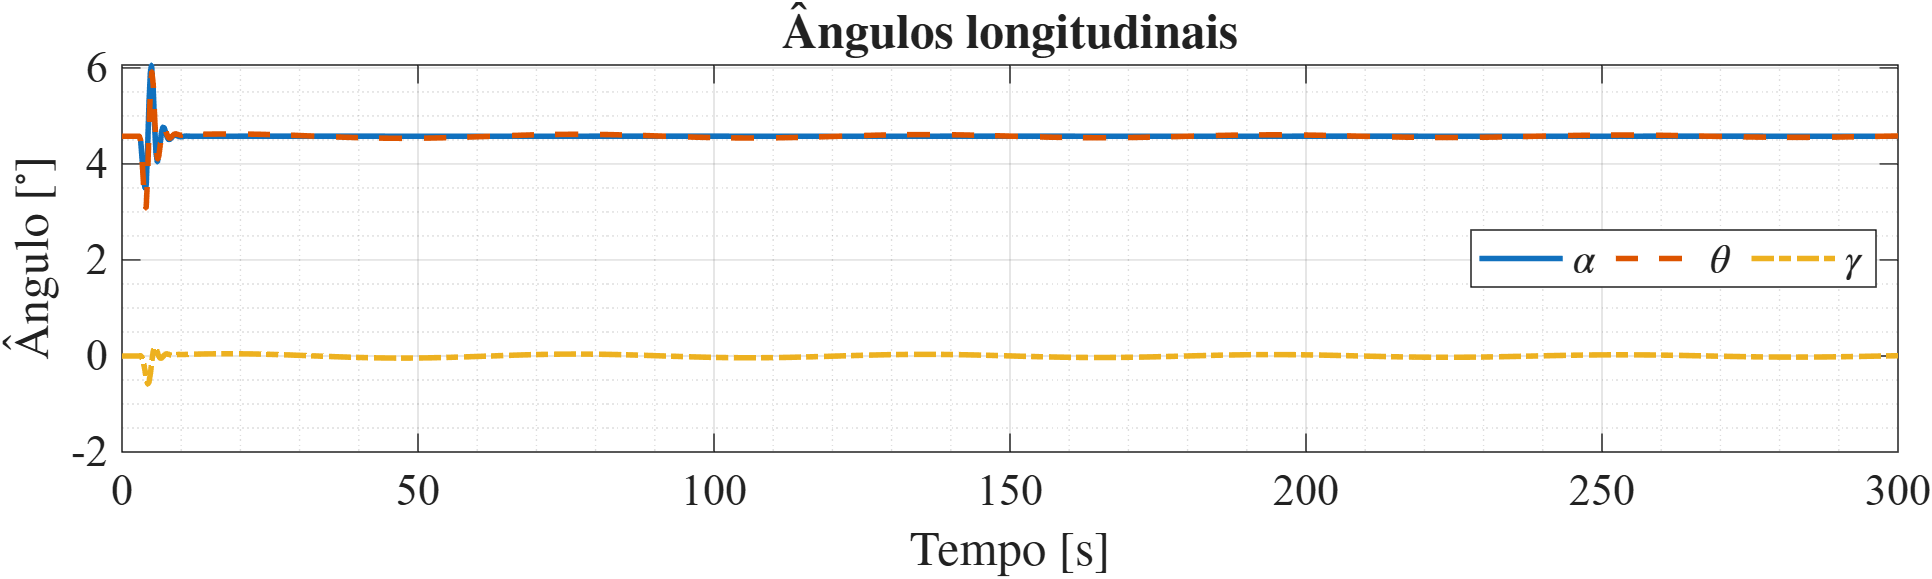
\includegraphics[width=0.9\linewidth]{images/estabilidade/angulos_300s_CG_dianteiro.png}
    \caption{Evolução de $\alpha$, $\theta$ e $\gamma$ para CG dianteiro}
    \label{fig:placeholder}
\end{figure}


\subsection{Derivadas de estabilidade}

\begin{table}[H]
    \centering
    \caption{Derivadas de estabilidade longitudinal e parâmetros associados para as condições extremas de CG, obtidas no AVL a 20000 ft de altitude.}
    \begin{tabular}{|l|c|c|}
       \hline
       \textbf{Parâmetro} & \textbf{CG dianteiro} & \textbf{CG traseiro} \\
       \hline
       $h_{CG}$ (\%  $\bar{c}$)        & $0{,}179$   & $0{,}459$  \\
       \hline
       Margem estática (SM)              & $0{,}561$   & $0{,}281$  \\
       \hline
       $C_{L_0}$                         & $0{,}1916$  & $0{,}1916$ \\
       \hline
       $C_{L_\alpha}$ [rad$^{-1}$]       & $5{,}816$   & $5{,}816$  \\
       \hline
       $C_{L_q}$ [rad$^{-1}$]            & $14{,}532$  & $11{,}274$ \\
       \hline
       $C_{L_\eta}$ [rad$^{-1}$]         & $0{,}636$   & $0{,}636$  \\
       \hline
       $C_{D_0}$                         & $0{,}00227$ & $0{,}00227$\\
       \hline
       $C_{m_0}$                         & $0{,}0150$  & $0{,}0687$ \\
       \hline
       $C_{m_\alpha}$ [rad$^{-1}$]       & $-3{,}265$  & $-1{,}636$ \\
       \hline
       $C_{m_q}$ [rad$^{-1}$]            & $-39{,}323$ & $-34{,}338$\\
       \hline
       $C_{m_\eta}$ [rad$^{-1}$]         & $-2{,}827$  & $-2{,}649$ \\
       \hline
    \end{tabular}
    \label{tab:derivadas_long_anexo}
\end{table}


\section{Dimensões Antropométricas de Pilotos}
\begin{table}[H]
    \centering
    \caption{Dimensões anatômicas estáticas detalhadas para ergonomia da cabine [cm].}
    \label{tab:dimensoes_anatomicas_cabine}
    \resizebox{\textwidth}{!}{%
    \begin{tabular}{lcccccc}
    \hline
        \textbf{Dimensão} &
        \multicolumn{3}{c}{\textbf{Masculino (M)}} &
        \multicolumn{3}{c}{\textbf{Feminino (F)}} \\
        \cline{2-7}
        & \textbf{5º} & \textbf{50º} & \textbf{95º}
        & \textbf{5º} & \textbf{50º} & \textbf{95º} \\
    \hline
        1 - Altura em posição sentada &
        85,8 & 91,4 & 97,2 & 79,5 & 85,1 & 91,0 \\

        2 - Altura dos olhos, sentado &
        73,5 & 79,2 & 84,8 & 68,5 & 73,8 & 79,4 \\

        3 - Altura do ombro, sentado &
        54,9 & 59,8 & 64,6 & 50,9 & 55,5 & 60,4 \\

        4 - Altura do cotovelo, sentado &
        18,4 & 23,2 & 27,4 & 17,6 & 22,1 & 26,4 \\

        5 - Espessura da coxa &
        14,9 & 16,8 & 19,0 & 14,0 & 15,8 & 18,0 \\

        6 - Altura do joelho, sentado &
        51,4 & 55,8 & 60,6 & 47,4 & 49,8 & 56,0 \\

        7 - Altura poplítea, sentado &
        39,5 & 43,3 & 47,6 & 35,1 & 38,9 & 42,9 \\

        8 - Comprimento antebraço-ponta do dedo &
        44,8 & 48,3 & 52,4 & 40,6 & 44,2 & 48,3 \\

        Alcance funcional do braço &
        73,9 & 80,0 & 86,7 & 67,7 & 73,4 & 79,7 \\

        9 - Largura dos ombros (bideltoide) &
        45,0 & 49,1 & 53,5 & 39,7 & 43,1 & 47,2 \\

        10 - Largura entre cotovelos &
        47,8 & 54,5 & 62,1 & 41,5 & 46,7 & 52,8 \\
    \hline
\end{tabular}%
}

\vspace{0.2cm}
\small Fonte: Adaptado de FAA HFDS \cite{FAA_HFDS}, Seção 5.12.3.2.
\end{table}

\section{Comparação entre Tecnologias de Freios}
\begin{table}[H]
    \centering
    \caption{Comparação entre tecnologias de freios aeronáuticos.}
    \vspace{0.2cm}

    \renewcommand{\arraystretch}{1.6}
    \setlength{\tabcolsep}{6pt}

    \begin{tabular}{|p{3.5cm}|p{3.2cm}|p{3.5cm}|p{5.2cm}|}
        \hline
        \textbf{Propriedade / Característica} &
        \textbf{Freios de Aço} &
        \textbf{Freios de Carbono} &
        \textbf{Impacto Técnico no Projeto} \\
        \hline

        Peso do Conjunto de Freios
        & Elevado (referência)
        & Redução de 35\% a 42\% em massa
        & Redução do OEW e aumento da capacidade de carga paga ou combustível \\
        \hline

        Condutividade Térmica
        & Moderada
        & Elevada
        & Dissipação térmica mais eficiente e menor risco de superaquecimento \\
        \hline

        Resistência Térmica e Vida Útil
        & Perda de eficiência acima de $500^\circ$C; vida útil entre 800 e 1200 ciclos
        & Operação estável até $1200^\circ$C; vida útil entre 1500 e 3000 ciclos
        & Maior confiabilidade operacional e redução de manutenção \\
        \hline

        Custo de Aquisição Inicial
        & Baixo
        & Elevado
        & Maior custo inicial compensado pela durabilidade e menor custo operacional \\
        \hline
    \end{tabular}

    \label{tab:comparacao_freios}
\end{table}

\section{Imagens Adicionais da Aeronave}
\begin{figure}[H] 
    \centering 
    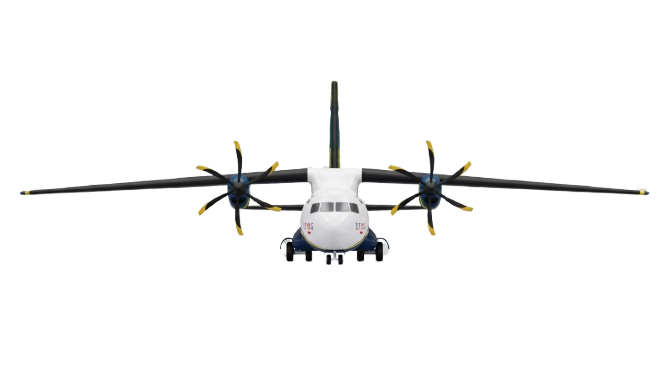
\includegraphics[width=1.00\textwidth]{Images-3-ProjetoDetalhado/Render_Frontal_v2.png} \caption{Vista frontal da configuração final da aeronave.} 
    \label{render_frontal} 
\end{figure}

% \begin{figure}[H] 
%     \centering 
%     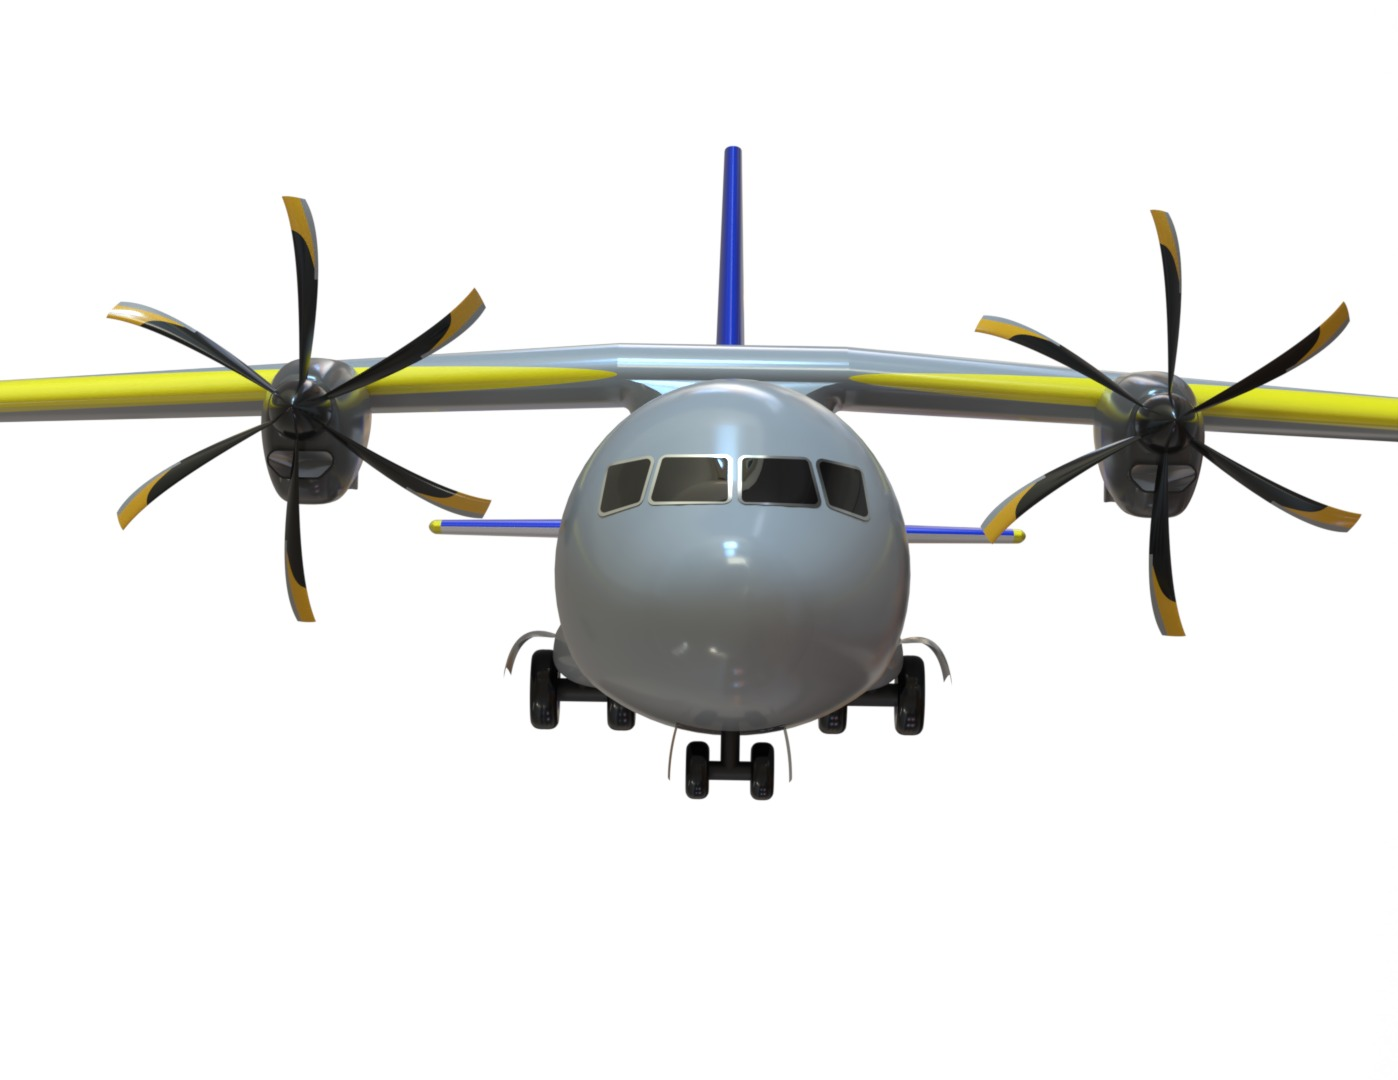
\includegraphics[width=0.85\textwidth]{Images-3-ProjetoDetalhado/render_frontal.jpeg} \caption{Renderização frontal da configuração final da aeronave.} 
%     \label{render_frontal} 
% \end{figure}

\begin{figure}[H] 
    \centering 
    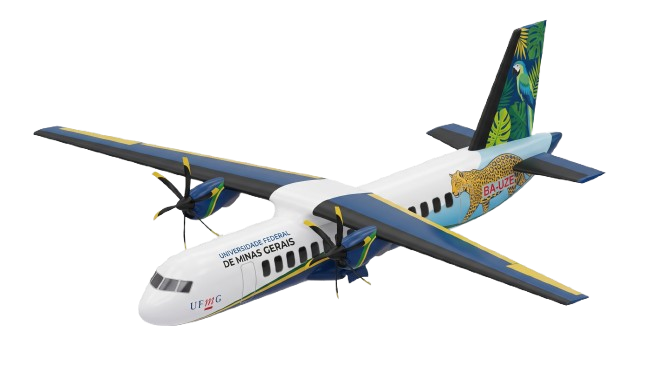
\includegraphics[width=1.0\textwidth]{Images-3-ProjetoDetalhado/render_isometrico.png} \caption{Vista em perspectiva da configuração final da aeronave.} 
    \label{render_frontal} 
\end{figure}

% \begin{figure}[H] 
%     \centering 
%     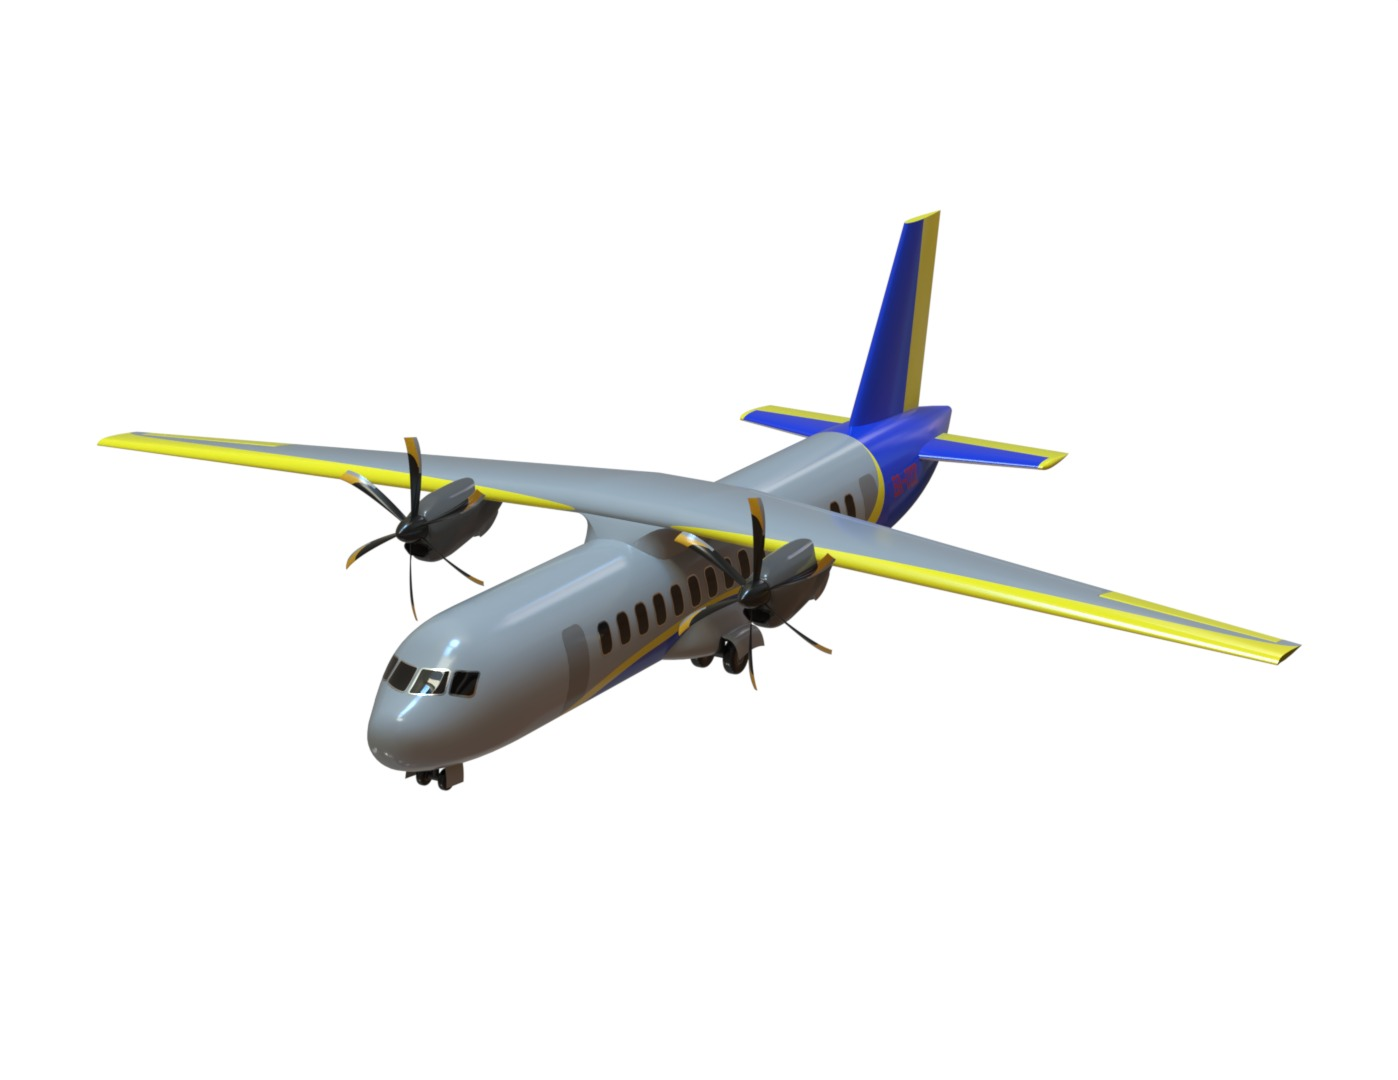
\includegraphics[width=1.0\textwidth]{Images-3-ProjetoDetalhado/render_perspectiva.jpeg} \caption{Renderização em perspectiva da configuração final da aeronave.} 
%     \label{render_frontal} 
% \end{figure}



\begin{figure}[H] 
    \centering 
    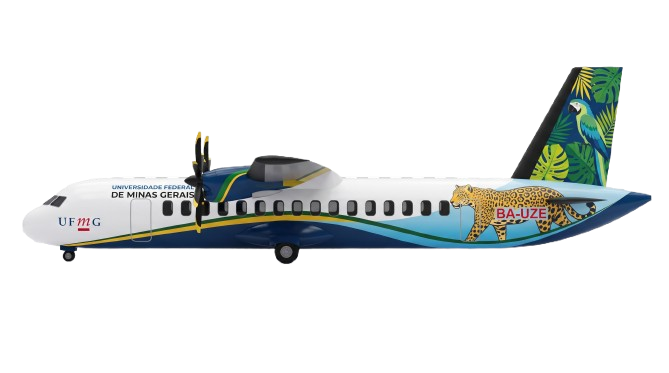
\includegraphics[width=1.0\textwidth]{Images-3-ProjetoDetalhado/render_lateral.jpeg} \caption{Vista Lateral da Aeronave} \label{render_lateral_dianteira} 
\end{figure}


% \begin{figure}[H] 
%     \centering 
%     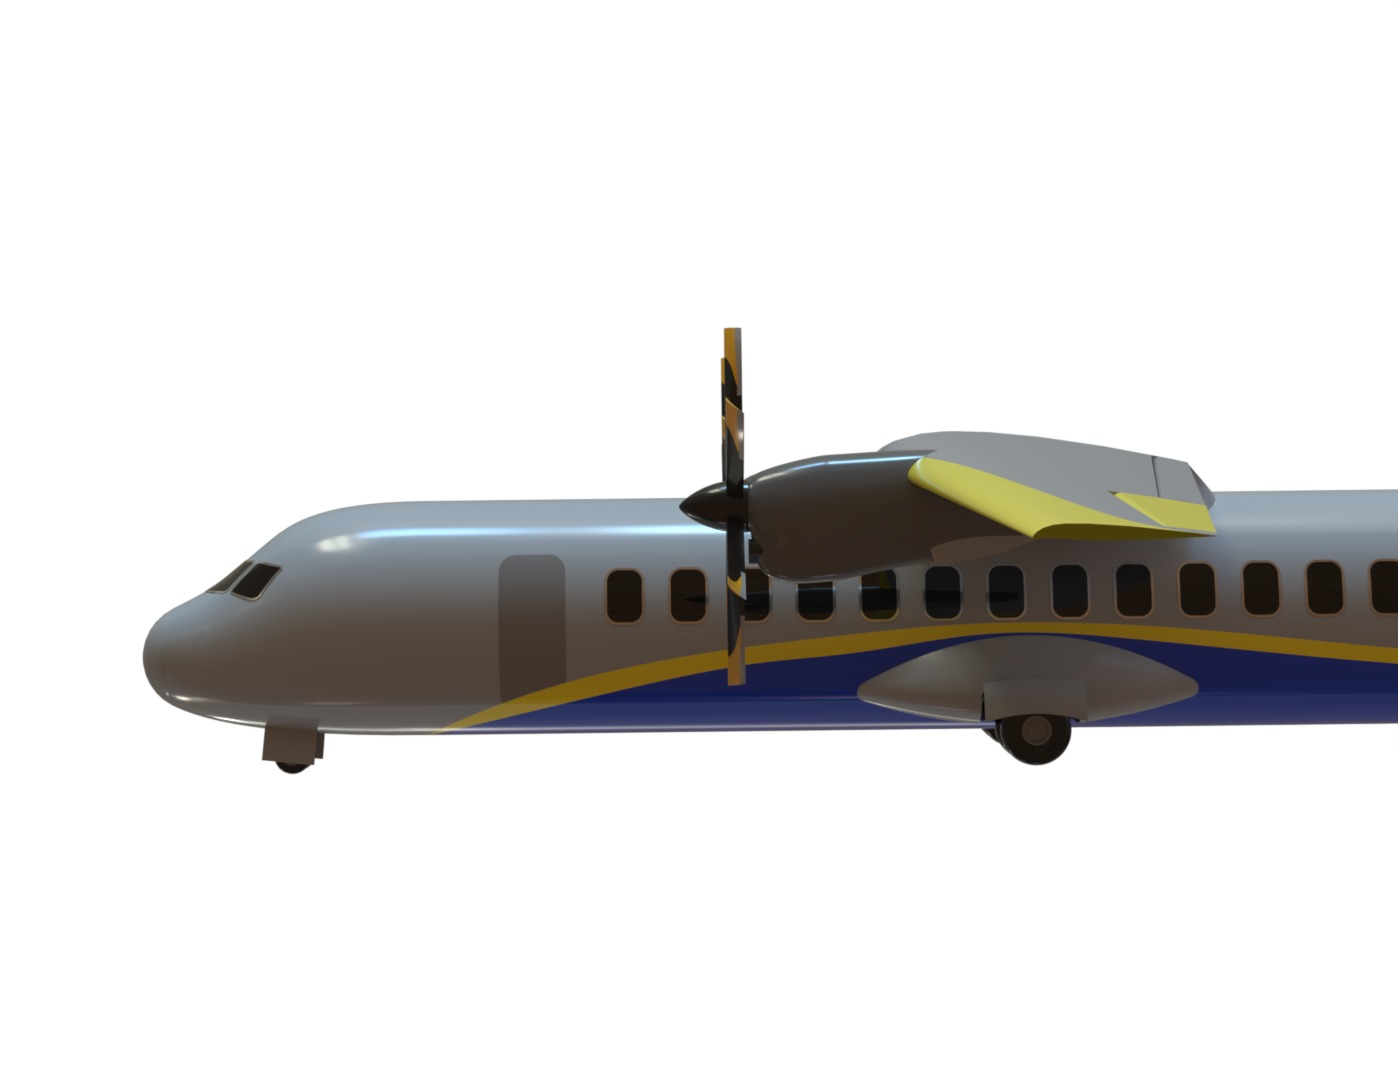
\includegraphics[width=0.68\textwidth]{Images-3-ProjetoDetalhado/render_lateral_dianteira.jpeg} \caption{Detalhe lateral dianteiro da aeronave, evidenciando a fuselagem, a nacele, o trem de pouso e a asa.} \label{render_lateral_dianteira} 
% \end{figure}

% \begin{figure}[H] 
%     \centering 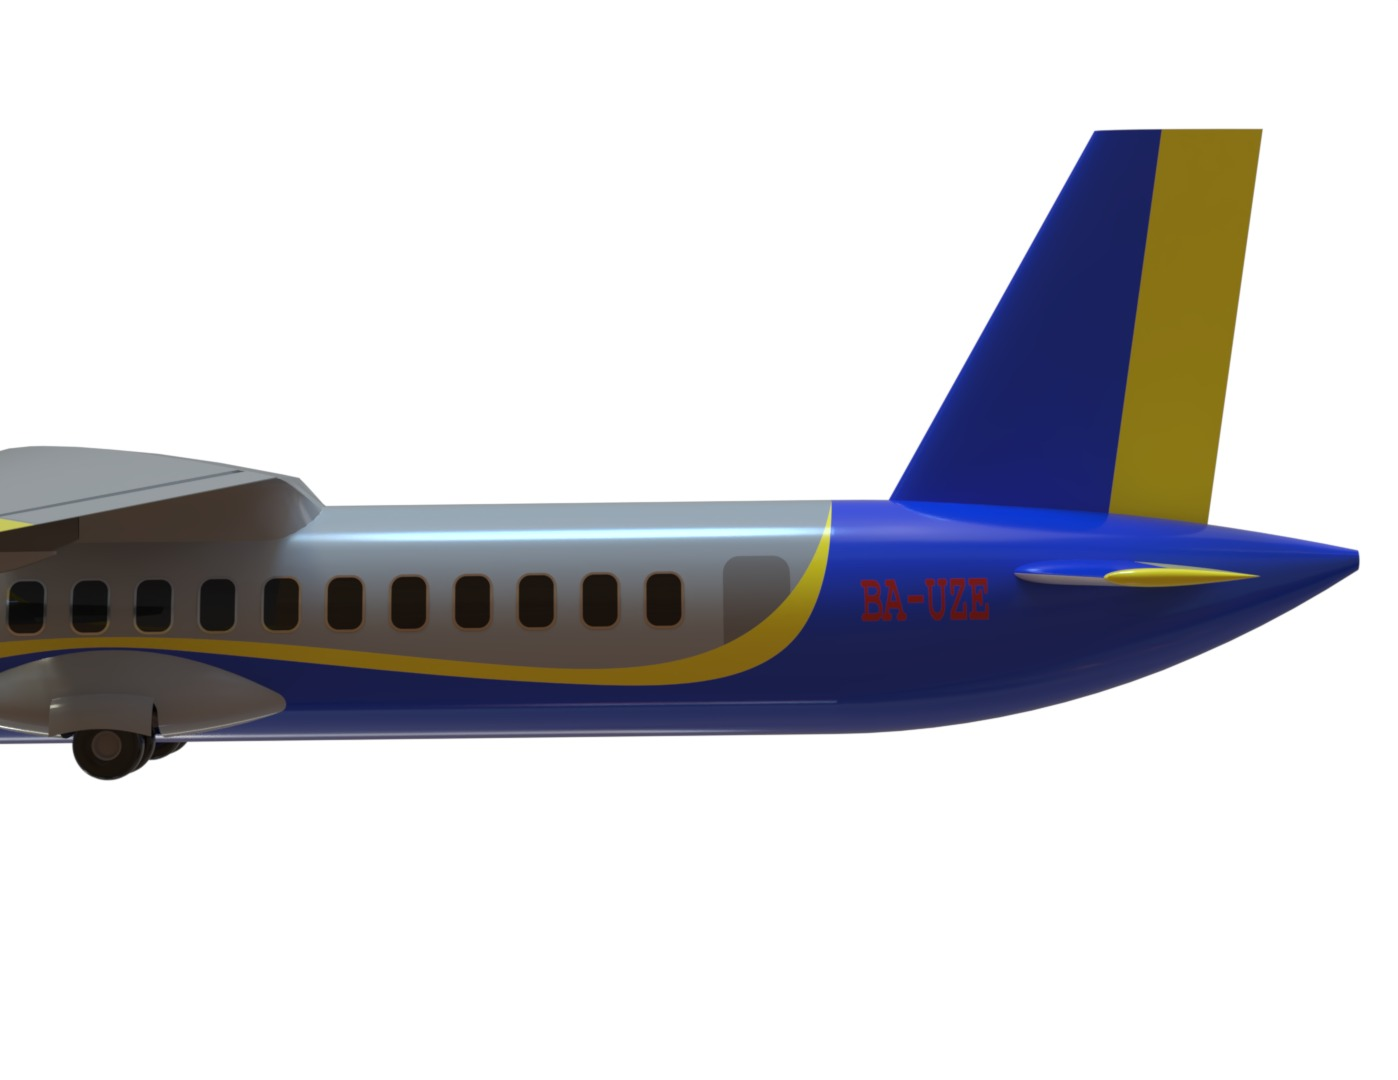
\includegraphics[width=0.68\textwidth]{Images-3-ProjetoDetalhado/render_traseira.jpeg} \caption{Detalhe da região traseira da aeronave, evidenciando as empenagens e o cone de cauda.} 
%     \label{render_traseira} 
% \end{figure} 


\subsection*{Projetos 1}

\begin{xltabular}{\textwidth}{|X|X|X|}
\caption{Distribuição de Responsabilidades por Seção -- Projetos 1} \label{tab:responsabilidades} \\

\hline
\textbf{Tópico} & \textbf{Execução} & \textbf{Revisão} \\
\hline
\endfirsthead % CORREÇÃO: Comando sem chavetas

\multicolumn{3}{c}{{\tablename\ \thetable{} -- Continuação da página anterior}} \\
\hline
\textbf{Tópico} & \textbf{Execução} & \textbf{Revisão} \\
\hline
\endhead % CORREÇÃO: Comando sem chavetas

\hline
\multicolumn{3}{r}{{Continua na próxima página...}} \\
\endfoot % CORREÇÃO: Comando sem chavetas

\hline
\endlastfoot % CORREÇÃO: Comando sem chavetas

% --- CONTEÚDO DA TABELA ---
Análise de mercado & Pedro Ornelas e Gabriel Soares & Carolina, Gabriela Machado, Gabriel Marques, Pedro Roquette, Rodrigo Vicente e Saulo Lacerda \\ \hline

Estudo Comparativo & Carolina, Gabriela Machado, Gabriel Marques, Pedro Roquette, Rodrigo e Vicente & Pedro Ornelas, Gabriel Soares e Saulo Lacerda \\
\hline

\multicolumn{3}{|c|}{\textbf{Projeto Conceitual}} \\
\hline

Geometria Interna & Carolina e Pedro Roquette & Gabriel Marques e Rodrigo \\ \hline

Geometria da Asa & Gabriela Machado & Gabriel Marques e Rodrigo \\ \hline

Geometria das Empenagens & Pedro Ornelas e Vicente & Gabriela Machado e Saulo Lacerda \\ \hline

Escolha de Propulsão & Gabriel Soares & Pedro Roquette\\ \hline

Estudo e Definição de Número de Pás de Hélice & Victor Teixeira & \\ \hline

Estimativa de pesos & Gabriel Soares & Gabriela Machado \\ \hline

Estimativa do CG & Carolina & Pedro Roquette \\ \hline

Esboços Iniciais & Gabriel Marques e Rodrigo & \\
\hline

\multicolumn{3}{|c|}{\textbf{Projeto Preliminar}} \\
\hline

Definição do Perfil da Asa & Rodrigo & Pedro Ornelas \\ \hline

Dimensionamento dos Flaps & Rodrigo & Pedro Ornelas \\ \hline

Geometria das Empenagens e Superfícies de Controle & Pedro Ornelas e Vicente & \\ \hline

Geometria Interna & Carolina e Saulo Lacerda & \\ \hline

Dimensionamento de Pneus e Freios & Gabriel Soares, Gabriela Machado e Filipe Gomes & \\ \hline

Aprofundamento do Estudo do CG & Carolina & Pedro Ornelas \\
\hline

\multicolumn{3}{|c|}{\textbf{Aerodinâmica e Desempenho}} \\
\hline

Cálculo estimado da Polar de Arrasto & Gabriel Marques e Vicente & \\ \hline

Cálculo das Potências & & Pedro Ornelas e Gabriel Marques \\ \hline

Velocidades máximas e mínimas & & Pedro Ornelas e Gabriel Marques \\ \hline

Distâncias de Decolagem e Pouso & Pedro Roquette & \\ \hline

Voo em curva & Pedro Roquette & Pedro Ornelas \\ \hline

Autonomia e Alcance & Pedro Roquette & Carolina \\ \hline

Envelope de Voo & Vicente & \\ \hline

Desempenho de Subida & Vicente & \\ \hline

Diagrama de Missão & & Carolina \\ \hline

Resumo dos Cálculos de Desempenho & Pedro Roquette & \\
\hline

Estabilidade longitudinal preliminar & Pedro Ornelas, Vicente & \\ \hline

\end{xltabular}

\subsection*{Projetos 2}

\begin{xltabular}{\textwidth}{|X|X|}
\caption{Distribuição de Responsabilidades por Seção -- Projetos 2}
\label{tab:responsabilidades_p2} \\

\hline
\textbf{Tópico} & \textbf{Execução} \\
\hline
\endfirsthead

\multicolumn{2}{c}{{\tablename\ \thetable{} -- Continuação da página anterior}} \\
\hline
\textbf{Tópico} & \textbf{Execução} \\
\hline
\endhead

\hline
\multicolumn{2}{r}{{Continua na próxima página...}} \\
\endfoot

\hline
\endlastfoot

% --- CONTEÚDO DA TABELA ---

Requisitos e Referências
& Luísa Vilela \\
\hline

Definição do Material
& Gabriel Soares \\
\hline

Revisão de Aerodinâmica
& Vitor Gonçalves e Pedro Roquette \\
\hline

Revisão de Desempenho
& Vitor Gonçalves, Pedro Roquette e Gabriel Marques\\
\hline

Revisão de Estabilidade e Controle
& Vicente Neto e Vitor Mendes \\
\hline

Revisão de Trem de Pouso e Sistemas
& Pedro Ornelas e Filipe Gomes \\
\hline

Ergonomia da Cabine
& Saulo Lacerda \\
\hline

Alterações na Geometria Externa
& Gabriela Machado e Caio Rickli \\
\hline

Cálculos de Peso e CG & Carolina Ferrari \\
\hline

Desenho da longarina, nervuras e vista em corte da fuselagem
& Gabriel Marques, Rodrigo Pena, Flaubert Ferreira, Victor Teixeira e Gabriel Soares \\
\hline

Cargas na Asa e Empenagens
& Vitor Gonçalves \\
\hline

Dimensionamento Estrutural
& Flaubert Ferreira \\
\hline

Dimensionamento do Revestimento
& Vitor Mendes \\
\hline

Materiais da Construção 
& Gabriel Soares e Saulo Lacerda \\
\hline

Dimensionamento do Berço do Motor 
& Gabriel Soares e Saulo Lacerda \\
\hline

\end{xltabular}

\includepdf[pages=-, angle=90]{detalhamento.pdf}

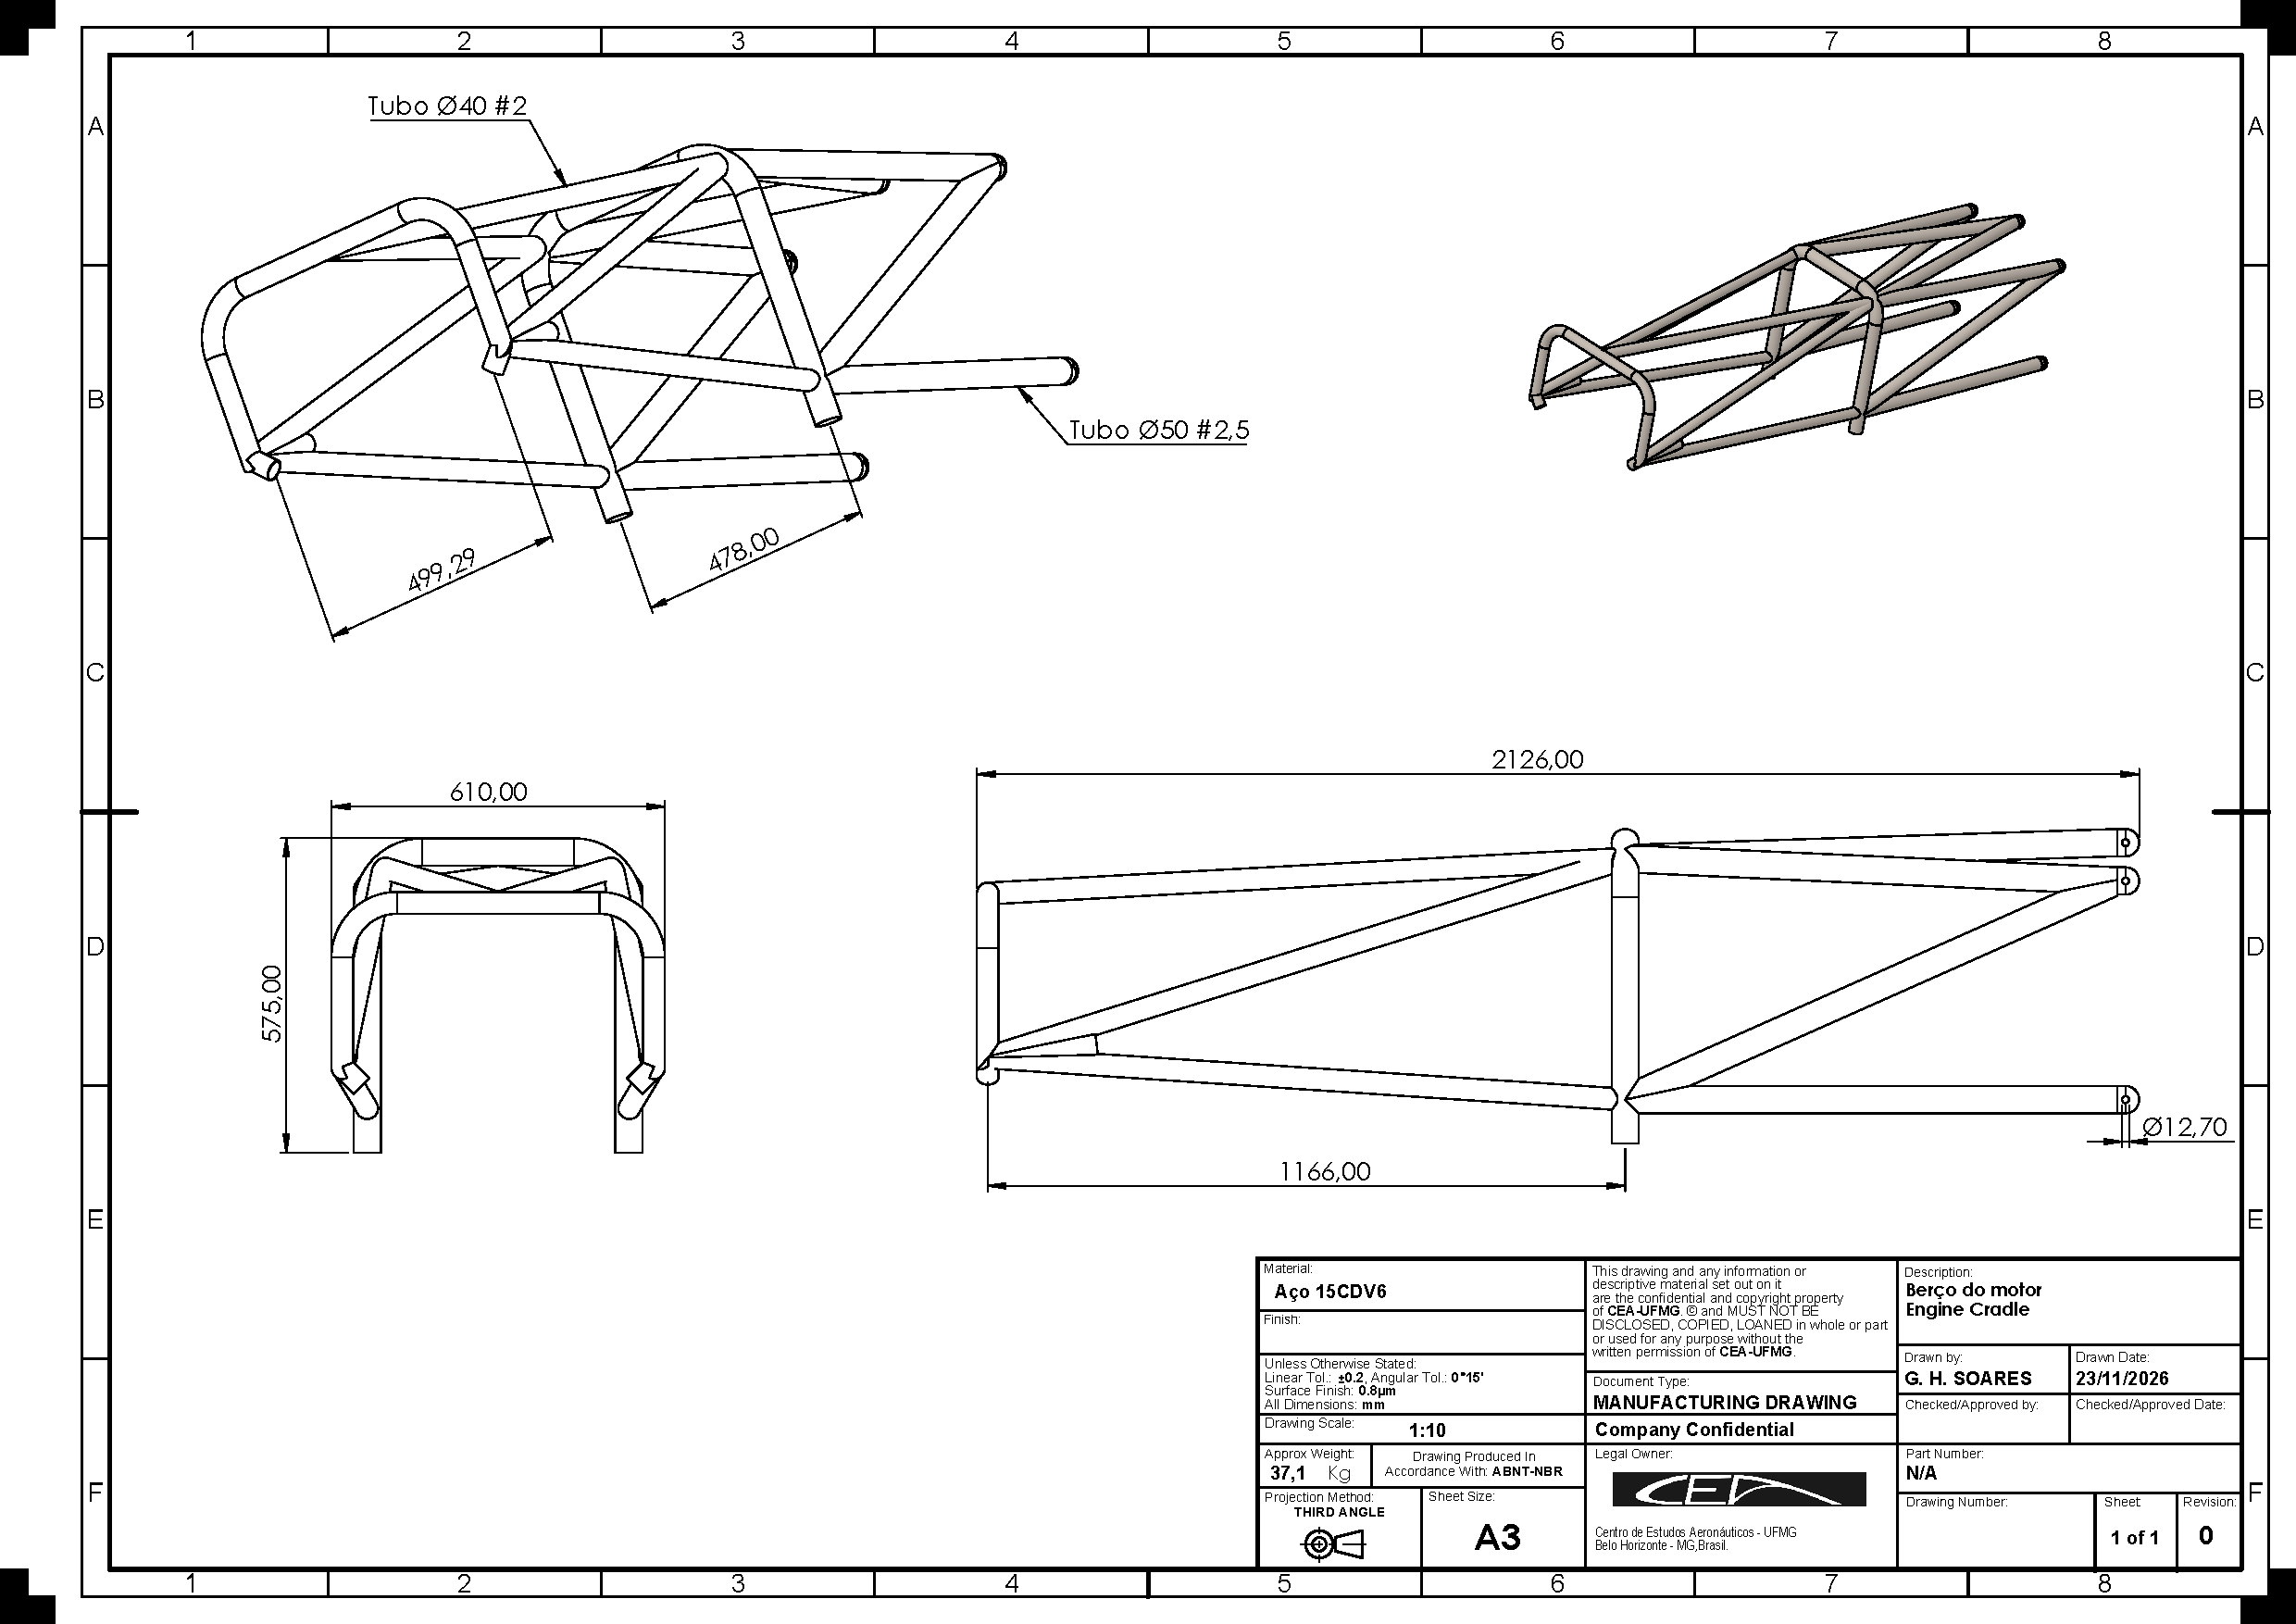
\includepdf[pages=-, angle=90]{berco.pdf}

